% =====================================================================
%  LUVE — Graduation Thesis
%  Tan Tao University — Faculty of Information Technology
%  Compile with: XeLaTeX  (Overleaf: Menu > Compiler > XeLaTeX)
%  Bibliography:  biber    (Overleaf auto-detects from biblatex)
%
%  LANGUAGE POLICY
%   - Thesis body language: ENGLISH. All visible text is in English.
%   - Internal image/table preparation notes for the student may stay in
%     Vietnamese, but ONLY inside "% TODO-FIGURE [VI]:" / "% TODO-TABLE [VI]:"
%     comments. These are never typeset into the PDF.
%   - All other comments (TODO-CITE, [PLACEHOLDER] guidance) are in English.
%
%  THESIS FOCUS
%   - This is a SOFTWARE / SYSTEM DESIGN thesis: architecture, component
%     responsibilities, data/control flow, real-time communication design,
%     backend/frontend integration, database and queue design, implementation
%     decisions, and runtime/devops constraints.
%   - Avoid over-emphasizing pedagogy theory, business value, marketing
%     claims, learner psychology, or unsupported learning-effectiveness
%     claims. Pedagogical terms appear only to name software features
%     (tutor reply, grading result, feedback display, session analysis).
%
%  This is a STRUCTURE-ONLY skeleton. Body text is placeholder notes only,
%  except §3.3.1 which is written. Resolve every [PLACEHOLDER ...],
%  TODO-FIGURE, TODO-TABLE, and TODO-CITE marker before submission.
% =====================================================================
% Note on font size: the standard `report` class only honours 10/11/12pt.
% We use 12pt (reliable on Overleaf XeLaTeX). If the faculty strictly
% requires 13pt, the stable way is to scale the whole document instead of
% asking `report` for an unsupported size — see the commented \setmainfont
% scale option below. Do NOT pass 13pt to \documentclass (it is silently
% ignored and makes the setup look fragile).
\documentclass[12pt,a4paper,oneside]{report}

% ---------- XeLaTeX language + font setup ---------------------------
\usepackage{fontspec}
\usepackage{polyglossia}
\setdefaultlanguage{english}
% Vietnamese kept as a secondary language only so any official Vietnamese
% administrative wording can still be typeset correctly if restored later.
\setotherlanguage{vietnamese}
% TeX Gyre Termes is a Times-compatible font (full Latin + Vietnamese
% coverage) available on Overleaf. Swap to "Times New Roman" only if you
% upload the font file to the project.
% For an effective ~13pt look, uncomment the Scale option (1.08 * 12pt):
% \setmainfont[Scale=1.08]{TeX Gyre Termes}
\setmainfont{TeX Gyre Termes}

% ---------- English names for auto-generated headings ---------------
\renewcommand{\contentsname}{TABLE OF CONTENTS}
\renewcommand{\listfigurename}{LIST OF FIGURES}
\renewcommand{\listtablename}{LIST OF TABLES}
\renewcommand{\bibname}{REFERENCES}
\renewcommand{\appendixname}{APPENDIX}

% ---------- Page geometry ------------------------------------------
\usepackage[a4paper,left=3cm,right=2cm,top=2cm,bottom=2cm]{geometry}

% ---------- Spacing -------------------------------------------------
\usepackage{setspace}
\onehalfspacing
\setlength{\parindent}{1cm}
\setlength{\parskip}{4pt}

% ---------- Common packages -----------------------------------------
\usepackage{graphicx}
\usepackage{booktabs}
\usepackage{longtable}
\usepackage{array}
\usepackage{caption}
\usepackage{float}
\usepackage{enumitem}
\usepackage{listings}      % code listings for the appendix
\usepackage{xcolor}

% ---------- Bibliography (IEEE style) -------------------------------
\usepackage[backend=biber,style=ieee,sorting=none]{biblatex}
\addbibresource{refs.bib}

% ---------- Hyperlinks (load late) ----------------------------------
\usepackage{hyperref}
\hypersetup{
  unicode=true,
  colorlinks=true,
  linkcolor=black,
  citecolor=black,
  urlcolor=blue,
  pdftitle={LUVE Graduation Thesis},
  pdfauthor={[PLACEHOLDER: Student full name]}
}

% ---------- Code listing style --------------------------------------
\lstset{
  basicstyle=\ttfamily\small,
  breaklines=true,
  frame=single,
  showstringspaces=false,
  columns=fullflexible
}

% ====================================================================
\begin{document}

% ===================== COVER PAGE ===================================
% NOTE: A Vietnamese university template usually prints the cover and
% approval pages in Vietnamese (official administrative wording). This
% thesis body is in English, so the institutional identity below is given
% in its official English form. If the faculty requires the Vietnamese
% originals, restore: Ministry of Education and Training / Tan Tao
% University / Faculty of Information Technology.
\begin{titlepage}
\centering
{\large MINISTRY OF EDUCATION AND TRAINING\par}
{\large TAN TAO UNIVERSITY\par}
{\large FACULTY OF INFORMATION TECHNOLOGY\par}
\vfill
{\Large\bfseries BACHELOR'S GRADUATION THESIS\par}
\vspace{1.5cm}
% TODO: confirm the official thesis title (uppercase, bold).
{\LARGE\bfseries LUVE: A REAL-TIME ENGLISH SPEAKING\\PRACTICE SYSTEM USING STT, LLM,\\AND AUTOMATED GRADING\par}
\vspace{1.5cm}
\begin{flushleft}
\hspace{3cm}\textbf{Major:} \quad [PLACEHOLDER: Major]\\[4pt]
\hspace{3cm}\textbf{Major code:} \quad [PLACEHOLDER: Major code]\\[4pt]
\hspace{3cm}\textbf{Cohort:} \quad [PLACEHOLDER: Intake year]\\[4pt]
\hspace{3cm}\textbf{Student:} \quad [PLACEHOLDER: Full name]\\[4pt]
\hspace{3cm}\textbf{Student ID:} \quad [PLACEHOLDER: Student ID]\\[4pt]
\hspace{3cm}\textbf{Supervisor:} \quad [PLACEHOLDER: Title, full name of supervisor]\\
\end{flushleft}
\vfill
{\large TAY NINH, MONTH [PLACEHOLDER] YEAR 20[PLACEHOLDER]\par}
\end{titlepage}

% ===================== APPROVAL PAGE ================================
\thispagestyle{empty}
\begin{center}
{\Large\bfseries APPROVAL PAGE\par}
\end{center}
\vspace{1cm}
This thesis has been presented and defended before the Graduation Thesis
Evaluation Committee.
\vspace{0.5cm}

Defense date: ....../....../20......

Result: ....../10 points
\vspace{2cm}

\noindent
\begin{minipage}[t]{0.32\textwidth}\centering
SUPERVISOR\\(Signature and full name)
\end{minipage}\hfill
\begin{minipage}[t]{0.32\textwidth}\centering
REVIEWER\\(Signature and full name)
\end{minipage}\hfill
\begin{minipage}[t]{0.32\textwidth}\centering
COMMITTEE CHAIR\\(Signature and full name)
\end{minipage}
\clearpage

% ===================== ACKNOWLEDGEMENTS ============================
\chapter*{ACKNOWLEDGEMENTS}
\addcontentsline{toc}{chapter}{ACKNOWLEDGEMENTS}
% [PLACEHOLDER] Acknowledge the supervisor, family, friends, and everyone
% who supported the thesis work.
I would like to sincerely thank [PLACEHOLDER: Supervisor's name] for the
dedicated guidance throughout this thesis. \ldots
\clearpage

% ===================== ABSTRACT ====================================
% A single English abstract is used (full-English thesis). If the faculty
% also requires a Vietnamese abstract, add a separate Vietnamese-abstract
% chapter (heading "TOM TAT LUAN VAN") in addition to this one.
\chapter*{ABSTRACT}
\addcontentsline{toc}{chapter}{ABSTRACT}
% [PLACEHOLDER] 200-300 words: objectives, methodology, main results,
% conclusions. Follow LUVE_FACTS.md - do NOT claim production-ready /
% stable multilingual STT / phoneme pronunciation scoring / exactly-once /
% horizontal scaling.
[PLACEHOLDER: English summary of the thesis.]
\vspace{0.5cm}

\noindent\textbf{Keywords:} [PLACEHOLDER: 4-6 keywords, comma-separated]
\clearpage

% ===================== TOC / LOF / LOT =============================
\tableofcontents
\clearpage
\listoffigures
\addcontentsline{toc}{chapter}{LIST OF FIGURES}
\clearpage
\listoftables
\addcontentsline{toc}{chapter}{LIST OF TABLES}
\clearpage

% ===================== ABBREVIATIONS ==============================
\chapter*{LIST OF ABBREVIATIONS}
\addcontentsline{toc}{chapter}{LIST OF ABBREVIATIONS}
\begin{longtable}{p{3cm} p{10cm}}
\toprule
\textbf{Abbreviation} & \textbf{Description} \\
\midrule
\endhead
AI     & Artificial Intelligence \\
ML     & Machine Learning \\
LLM    & Large Language Model \\
STT    & Speech-to-Text \\
TTS    & Text-to-Speech \\
VAD    & Voice Activity Detection \\
WebRTC & Web Real-Time Communication \\
API    & Application Programming Interface \\
REST   & Representational State Transfer \\
SQL    & Structured Query Language \\
DLQ    & Dead Letter Queue \\
% [PLACEHOLDER] Add more abbreviations as needed.
\bottomrule
\end{longtable}
\clearpage

% ===================== MAIN MATTER ================================

% ------------------- CHAPTER 1 ------------------------------------
\chapter{INTRODUCTION}

\section{Problem Statement}
% [PLACEHOLDER] Background, motivation, and significance of the topic.
% TODO-CITE: demand for English speaking practice / limitations of traditional methods.

\section{Research Objectives}
\subsection{General Objective}
% [PLACEHOLDER] Overall goal: build a real-time English speaking practice
% demo system (STT + LLM tutor + grading of saved sessions).

\subsection{Specific Objectives}
% [PLACEHOLDER] Specific objectives, following LUVE_FACTS.md.

\section{Research Subject and Scope}
\subsection{Research Subject}
% [PLACEHOLDER]
\subsection{Research Scope}
% [PLACEHOLDER] State clearly: this is a controlled-demo / research prototype,
% NOT a production product. STT stable mode: forced_en + small.en, second-pass
% disabled by default.

\section{Research Methodology}
% [PLACEHOLDER]

\section{Scientific and Practical Significance}
% [PLACEHOLDER]

\section{Thesis Structure}
% [PLACEHOLDER] Briefly describe the five chapters.

% ------------------- CHAPTER 2 ------------------------------------
\chapter{THEORETICAL BACKGROUND AND RELATED WORK}

\section{Related Concepts}
% [PLACEHOLDER] STT, LLM, TTS, VAD, WebRTC, message queue, outbox pattern.

\section{Theoretical Foundation}
% [PLACEHOLDER]
% TODO-CITE: Whisper / faster-whisper.
% TODO-CITE: Large Language Models.
% TODO-CITE: WebRTC.
% TODO-CITE: transactional outbox pattern.

\section{Review of Related Work}
\subsection{Domestic Studies}
% [PLACEHOLDER]
% TODO-CITE
\subsection{International Studies}
% [PLACEHOLDER]
% TODO-CITE

\section{Technologies Used}
% [PLACEHOLDER] FastAPI, Docker Compose, PostgreSQL, RabbitMQ,
% faster-whisper (small.en), LLM tutor (Groq), Vite/React client.
% See LUVE_FACTS.md for the exact names/configuration.

\section{Chapter Summary}
% [PLACEHOLDER]

% ------------------- CHAPTER 3 ------------------------------------
\chapter{RESEARCH METHODOLOGY AND SYSTEM DESIGN}

\section{Research Methodology}
% [PLACEHOLDER]

\section{Requirements Analysis}
\subsection{Functional Requirements}
% [PLACEHOLDER] Real-time speaking practice; STT; LLM tutor replies;
% session saving; grading of saved sessions.
\subsection{Non-functional Requirements}
% [PLACEHOLDER] Privacy (transcripts redacted from logs), security
% (locked CORS, session-ownership check), reliability (durable outbox).

\section{System Design}
\subsection{System Architecture}

LUVE is built as a research prototype for real-time English speaking
practice. The version presented in this thesis corresponds to the frozen
source-code baseline \texttt{main@6a61bc8}. The system is organized as a
multi-service application running under Docker Compose, in which the
services communicate with one another only through two channels: the HTTP
protocol and the RabbitMQ message queue. This organization cleanly separates
the real-time conversation flow from the asynchronous grading flow, allowing
one component to be developed or replaced without directly affecting the
others.

% TODO-FIGURE [VI]: fig/architecture_overview — Hình 3.1: Kiến trúc tổng thể LUVE.
% Sơ đồ BẮT BUỘC phải thể hiện đầy đủ các thành phần và quan hệ:
%   - Client (trình duyệt, ứng dụng Vite/React)
%   - Core API (FastAPI REST, main.py, cổng 8000)
%   - TEN/WebRTC realtime gateway (run_ten.py, cổng 8080)
%   - STT (faster-whisper small.en, forced_en)
%   - LLM tutor (sinh phản hồi hội thoại thời gian thực)
%   - PostgreSQL
%   - RabbitMQ
%   - grading-worker
%   - session_outbox: là một BẢNG trong PostgreSQL (ghi cùng transaction với
%     sessions), KHÔNG phải một dịch vụ hàng đợi độc lập. Bộ chuyển tiếp
%     (relay) của outbox mặc định TẮT (default-off) và chỉ chạy thủ công khi
%     được bật.
% Mũi tên cần phân biệt: luồng thời gian thực (Client <-> gateway qua WebRTC)
% và luồng bất đồng bộ (session.completed qua RabbitMQ -> grading-worker).
\begin{figure}[H]
  \centering
  % 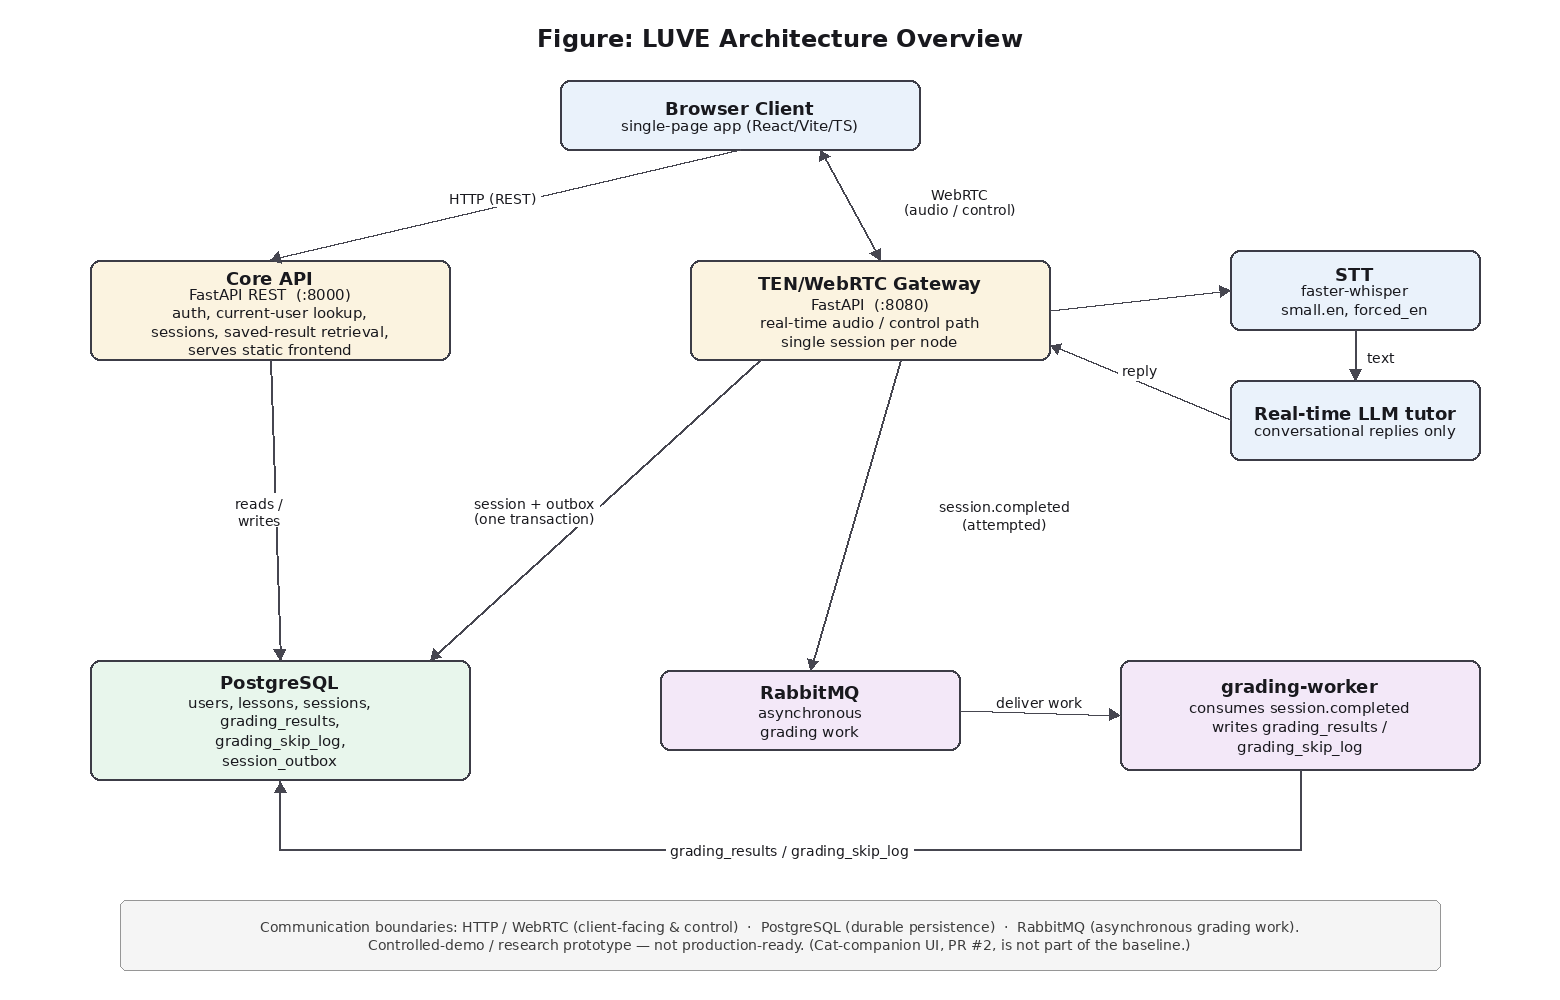
\includegraphics[width=\textwidth]{fig/architecture_overview.png}
  \caption{Overall architecture of the LUVE system.}
  \label{fig:arch}
\end{figure}

Figure~\ref{fig:arch} shows the overall architecture of LUVE. The system
comprises the following main components:

\begin{itemize}[leftmargin=*]
  \item \textbf{Client application.} This is the browser-based interface
  where the learner starts a practice session, speaks into the microphone,
  and receives the virtual tutor's replies as well as the grading results
  of saved sessions. Note that the ``cat companion'' interface (PR~\#2) has
  not been merged into \texttt{main} and is therefore not considered part of
  the baseline architecture in this thesis.

  \item \textbf{Core API.} A FastAPI service (file \texttt{main.py}, port
  8000) responsible for REST functions such as authentication, user
  management, and session management. It is the entry point for operations
  that are not part of the real-time audio path.

  \item \textbf{Real-time TEN/WebRTC gateway.} A second FastAPI application
  (file \texttt{run\_ten.py}, port 8080) that shares the same codebase as
  the Core API but serves the real-time conversation path exclusively. This
  gateway establishes the WebRTC connection with the browser, receives the
  learner's audio stream, and orchestrates the processing steps on the
  ``hot path''. The path is capped at a single session per node
  (\textit{single-session-per-node}).
  % TODO-CITE: Need an official source for WebRTC as a browser real-time communication standard.

  \item \textbf{Speech-to-Text (STT) component.} LUVE uses the
  \texttt{faster-whisper} model with the stable demo configuration
  \texttt{small.en} in \texttt{forced\_en} mode (forced English
  recognition), and the second-pass verification step is disabled by
  default. The STT component converts the learner's audio into text together
  with confidence metrics.
  % TODO-CITE: faster-whisper / Whisper (Radford et al.).

  \item \textbf{Tutor response component (LLM tutor).} The recognized text
  is fed into a large language model to generate a conversational reply for
  the learner. In the real-time flow, the large language model is used to
  generate conversational replies appropriate to the context of the
  learner's utterance. This component is not described as the primary grader;
  the full pedagogical evaluation and grading results are processed
  asynchronously by the grading-worker after the session ends. This component
  provides the ``tutor'' behavior of the system.
  % TODO-CITE: the large language model used for the tutor component.

  \item \textbf{PostgreSQL database.} Stores the system's persistent data,
  including users, lessons, practice sessions, and grading results. In
  particular, the database contains the \texttt{session\_outbox} table that
  supports the reliable event-delivery mechanism (described later).

  \item \textbf{RabbitMQ message queue.} Acts as the asynchronous channel
  between the conversation flow and the grading flow. When a session ends,
  the \texttt{session.completed} event is delivered through RabbitMQ to
  trigger the grading process.

  \item \textbf{Grading service (grading-worker).} A consumer process that
  listens on the \texttt{luve.session.completed} queue. It performs grading
  for the completed session and writes the results back to the database for
  later display.
\end{itemize}

% TODO-TABLE [VI]: Bảng 3.1 - Trách nhiệm các module hệ thống. Nội dung cần có:
% tên module (core-api main.py, core-api run_ten.py, grading-worker), cổng/giao
% tiếp, trách nhiệm chính. Bám LUVE_FACTS.md (hai service chỉ giao tiếp HTTP+RabbitMQ).

\textbf{Main data and control flow.} A typical practice session proceeds as
follows. First, the learner speaks into the microphone in the browser; the
real-time audio stream is transported to the TEN/WebRTC gateway over the
WebRTC connection. There, the STT component converts the audio into
recognized text. This text is passed to the LLM tutor component to generate
a conversational reply appropriate to the context, which is then played back
to the learner. Session events are collected during the interaction and
persisted when the session ends. At session completion, the system writes
the session record and a \texttt{session\_outbox} record within the same
database transaction, then publishes the \texttt{session.completed} event. If
the process crashes before session completion, part of the event log still
held in memory may not have been persisted; this is a limitation of the
current prototype. The \texttt{session.completed} event is delivered to the
grading flow through RabbitMQ; the grading-worker receives it, performs
grading, and stores the results in the database for later display to the
learner.

\textbf{Boundary between real-time conversation and asynchronous grading.}
An important design characteristic of LUVE is the clear separation between
the two flows. The real-time conversation flow (between the browser and the
TEN/WebRTC gateway) requires low latency and runs online, whereas the grading
flow is asynchronous and does not sit on the hot path. Grading is triggered
only after the session has ended, through the message queue. Thanks to this
boundary, the latency or computational load of the grading stage does not
affect the learner's conversation experience. The event-delivery mechanism
uses the durable \textit{outbox} pattern: the outbox record is written in the
same transaction as the session record, so it is not lost once the
transaction succeeds. However, in the current version the outbox
\textit{relay} is disabled by default, so recovery after a failed event
publish is a manual operation unless the relay is enabled. Message delivery
is \textit{at-least-once}, and the grading process is designed to be
idempotent through deduplication on \texttt{session\_id}; therefore the
system does not claim exactly-once delivery guarantees.
% TODO-CITE: the transactional outbox design pattern.

\textbf{Privacy and security notes.} The real-time session control routes,
specifically \texttt{/rtc/offer}, \texttt{/rtc/ice}, and \texttt{/rtc/cmd},
are protected by a session-ownership check: only the legitimate owner of a
session may operate on it. However, not every gateway endpoint is protected:
the health and diagnostic endpoints return only operational metadata and
remain a security hardening limitation. In addition, after the privacy patch
PR~\#1 (merged into \texttt{main}), the log records no longer store the
learner's raw recognized text; instead, the logs keep only metadata such as
text length and confidence metrics. This is an improvement in user-data
protection during experimental operation.

\textbf{Prototype limitation.} It must be emphasized that the architecture
above is designed for a controlled demo serving research purposes, not for
production-scale deployment. The real-time path is capped at a single session
per node, and the system has not demonstrated horizontal scaling. These
limitations are analyzed in more detail in Chapter~5.

% TODO-FIGURE [VI]: fig/realtime_pipeline — đường ống hot-path
% VAD -> STT -> LLM -> TTS -> WebRTC.
\begin{figure}[H]
  \centering
  % 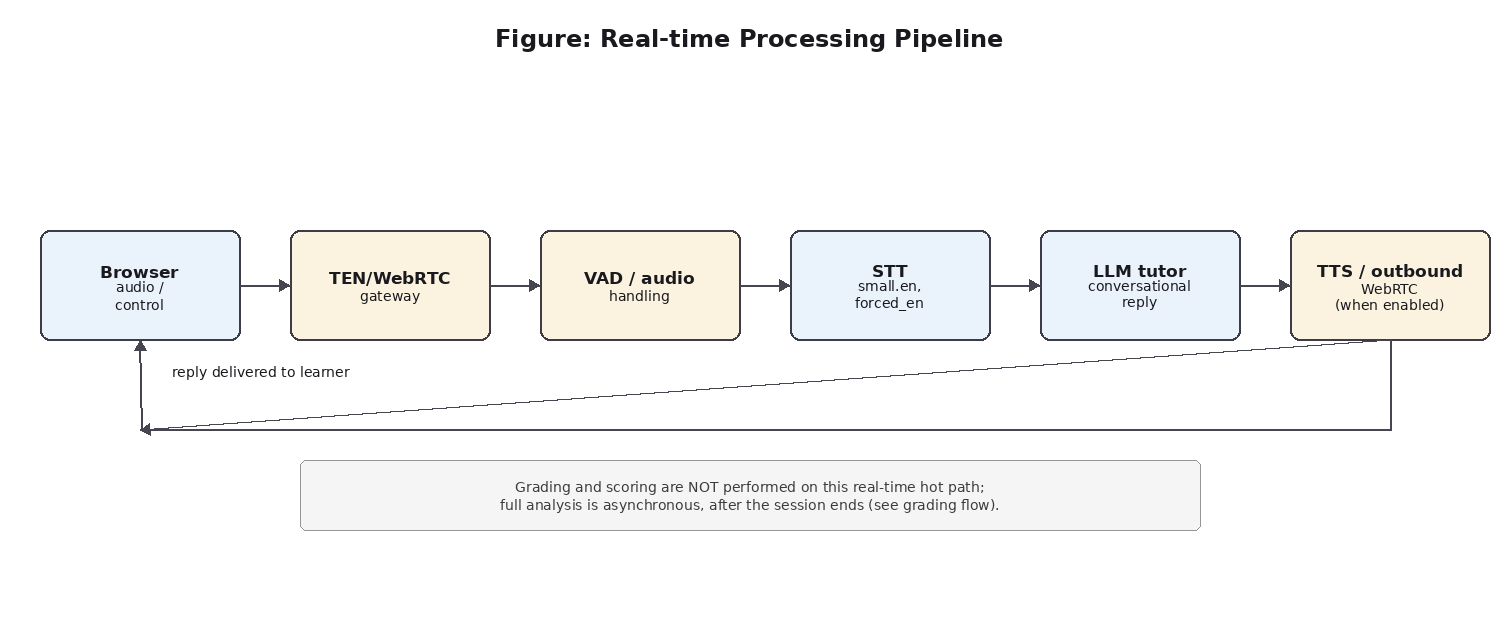
\includegraphics[width=\textwidth]{fig/realtime_pipeline.png}
  \caption{Real-time processing pipeline (VAD $\to$ STT $\to$ LLM $\to$ TTS $\to$ WebRTC).}
  \label{fig:pipeline}
\end{figure}

\subsection{Database Design}

LUVE uses PostgreSQL as the single durable state store for the system. A
relational database is appropriate here because the application's core
entities --- accounts, practice sessions, and grading outcomes --- have
well-defined relationships and benefit from transactional guarantees. In
particular, the session-completion step must update session state and record
an outbound grading event together as an atomic unit; PostgreSQL's
transactional semantics make this possible within a single commit, which is
the foundation of the reliability design discussed below. The schema is
defined in the baseline initialization script and evolved through a small set
of numbered SQL migration files (no object-relational mapping migration tool
is used).

% TODO-FIGURE [VI]: Cần vẽ ERD cơ sở dữ liệu chính của LUVE, gồm users, lessons, sessions, grading_results, grading_skip_log, session_outbox và quan hệ chính giữa chúng.
\begin{figure}[H]
  \centering
  % 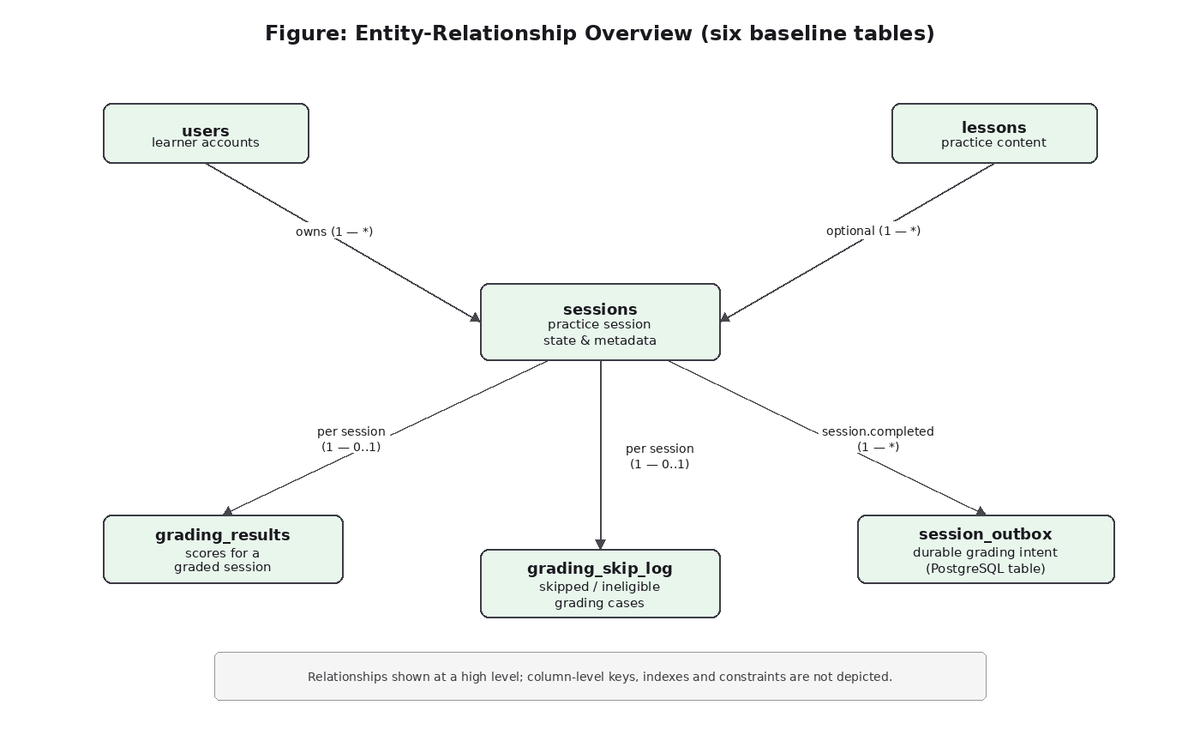
\includegraphics[width=\textwidth]{fig/erd.png}
  \caption{Entity-relationship diagram (ERD) of the LUVE database.}
  \label{fig:erd}
\end{figure}

Figure~\ref{fig:erd} shows the entity-relationship structure of the LUVE
database. The baseline schema (\texttt{main@6a61bc8}) contains six tables,
each with a distinct responsibility:

\begin{itemize}[leftmargin=*]
  \item \texttt{users} --- authenticated account records for learners. This
  table is the identity anchor of the system; other records that belong to a
  user reference it.

  \item \texttt{lessons} --- metadata for lesson or practice content. It acts
  as the catalogue of practice material that a session may be associated with
  in the baseline schema.

  \item \texttt{sessions} --- the lifecycle and metadata of a practice
  session. A session row captures the state of a speaking session and the
  information needed after it ends, including its completion status, a backup
  of the session payload (\texttt{raw\_backup\_json}), and the end timestamp
  (\texttt{ended\_at}). This table is the central record around which the
  grading pipeline is organized.

  \item \texttt{grading\_results} --- the persisted grading output for a
  completed session. It stores the overall and per-skill scores
  (fluency, grammar, vocabulary, and a pronunciation-clarity score) together
  with structured per-skill feedback (\texttt{skill\_feedback\_json}) and
  provenance fields such as the scoring-schema version, the grading provider,
  and the grader version. The pronunciation-clarity score is a clarity
  estimate derived from speech-recognition confidence, not an acoustic or
  phoneme-level pronunciation score.

  \item \texttt{grading\_skip\_log} --- a record of cases in which grading was
  skipped, together with the reason. This captures sessions that did not meet
  the eligibility conditions for grading, so that skipped cases remain
  observable rather than silently disappearing.

  \item \texttt{session\_outbox} --- a durable outbox table that bridges
  session completion and the asynchronous delivery of the grading event. It
  is a regular PostgreSQL table, written within the same transaction as the
  session record, and is \emph{not} a standalone queue service.
\end{itemize}

% TODO-TABLE [VI]: Cần lập bảng tóm tắt các bảng dữ liệu chính: tên bảng, trách nhiệm, dữ liệu chính, quan hệ liên quan.

\textbf{Relationships between tables.} The principal relationships follow the
lifecycle of a practice session. In the application flow, sessions belong to
authenticated users; at the schema level, \texttt{sessions.user\_id}
references \texttt{users.id}, while the implementation remains tolerant of
nullable session ownership in some records. Each completed \texttt{sessions}
record is associated with the grading artefacts it produces:
\texttt{grading\_results.session\_id} and \texttt{grading\_skip\_log.session\_id}
are each unique per session in their respective tables. A
\texttt{grading\_results} row holds the scores for a graded session, while a
\texttt{grading\_skip\_log} row can record cases where grading is skipped or
cannot proceed; the schema does not need to be described as enforcing a
cross-table exclusive choice between the two. The asynchronous delivery
boundary is represented by \texttt{session\_outbox}, where a row corresponds
to the \texttt{session.completed} event of a given session. A session may be
tied to specific practice material: \texttt{sessions.lesson\_id} is optional
and references \texttt{lessons.id}; if a lesson is deleted, the session record
can remain with \texttt{lesson\_id} set to \texttt{NULL}. Grading-related rows
are keyed so that the grading process can be deduplicated on the session
identifier.

\textbf{Support for the runtime flow.} The schema mirrors the end-to-end
runtime sequence described in Section~3.3.1. The real-time speaking session
occurs first, on the conversation path; during the interaction, session
events are accumulated. Durable session state is persisted only at completion:
when the session ends, the system writes the \texttt{sessions} row and a
\texttt{session\_outbox} row in one database transaction, and the
\texttt{session.completed} event is then delivered across the queue boundary.
Later, and off the real-time path, the grading-worker consumes that event and
writes the resulting \texttt{grading\_results} (or a \texttt{grading\_skip\_log}
entry when grading is skipped). The application uses the schema to persist the
main runtime stages in order: live session $\rightarrow$ durable session state
$\rightarrow$ outbox event $\rightarrow$ grading result.

\textbf{Reliability design.} The \texttt{session\_outbox} table is the core of
the reliability boundary between the synchronous session and the asynchronous
grading pipeline. Because the outbox row is committed in the same transaction
as the session record, the intent to grade a completed session is captured
durably even if the subsequent message publish to RabbitMQ fails. In the
current baseline the inline publish is the live delivery path, and the outbox
relay that would automatically re-deliver pending rows is disabled by default;
recovery from a failed publish is therefore a manual operation unless the
relay is enabled. The design is oriented toward at-least-once delivery, and
grading is idempotent through deduplication on the session identifier, so a
re-delivered event does not produce duplicate results. The system does not
provide, and this thesis does not claim, exactly-once delivery.

\textbf{Privacy and design notes.} The persisted session and grading data are
deliberately kept separate from application logs. Following the backend
privacy patch (PR~\#1, merged into \texttt{main}), raw recognized transcripts
are redacted from the logs --- the logs retain only metadata such as text
length and confidence values. Raw transcript text is thus not treated as
persistent application logging; the durable record of a session lives in the
database tables described above rather than in log output.

\textbf{Limitations.} The schema is created from a baseline initialization
script and evolved through numbered SQL migration files, but the current
baseline has no production-grade automatic migration runner; migrations are
manual SQL files with manual verification and readiness checks. As a
consequence, a database volume that predates a migration may
require manual verification that the migration has been applied before the
corresponding feature behaves correctly. In addition, because durable session
state is written only at completion, a process crash before completion may
lose the portion of the session event log still held in memory. These
constraints are consistent with the controlled-demo, research-prototype scope
of the system and are revisited in Chapter~5.

\subsection{Interface Design}

The interface is the presentation layer of LUVE and the learner's entry point
to the system. It is a frontend client that sits on top of the two backend
surfaces described earlier: the Core API for authentication, session
management, and saved-session review, and the real-time gateway for the
WebRTC audio and control flow of a live session. The interface does not
implement application logic of its own beyond presentation and orchestration;
it exposes system capabilities by calling the backend contracts and rendering
their responses. This section describes the baseline client (\texttt{main@6a61bc8})
at the design level; the unmerged ``cat companion'' interface (PR~\#2) is not
part of the baseline and is not treated as an implemented feature here.

\textbf{Authentication and session ownership.} The interface distinguishes an
unauthenticated state from an authenticated one. Unauthenticated users are
limited to the introductory and authentication entry points, including
sign-in and account creation, while the practice and review screens are
available only after authentication. Once signed in, the client issues
user-scoped API calls and operates within the backend's session-ownership
model, so that a learner can act only on their own sessions; the real-time
control routes are likewise guarded by the same ownership check on the gateway.
The interface therefore mirrors, at the presentation layer, the access
boundaries that the backend enforces.

% TODO-FIGURE [VI]: Cần chụp màn hình giao diện đăng nhập/khởi tạo phiên học từ baseline main, không dùng PR #2 cat companion UI.
\begin{figure}[H]
  \centering
  % 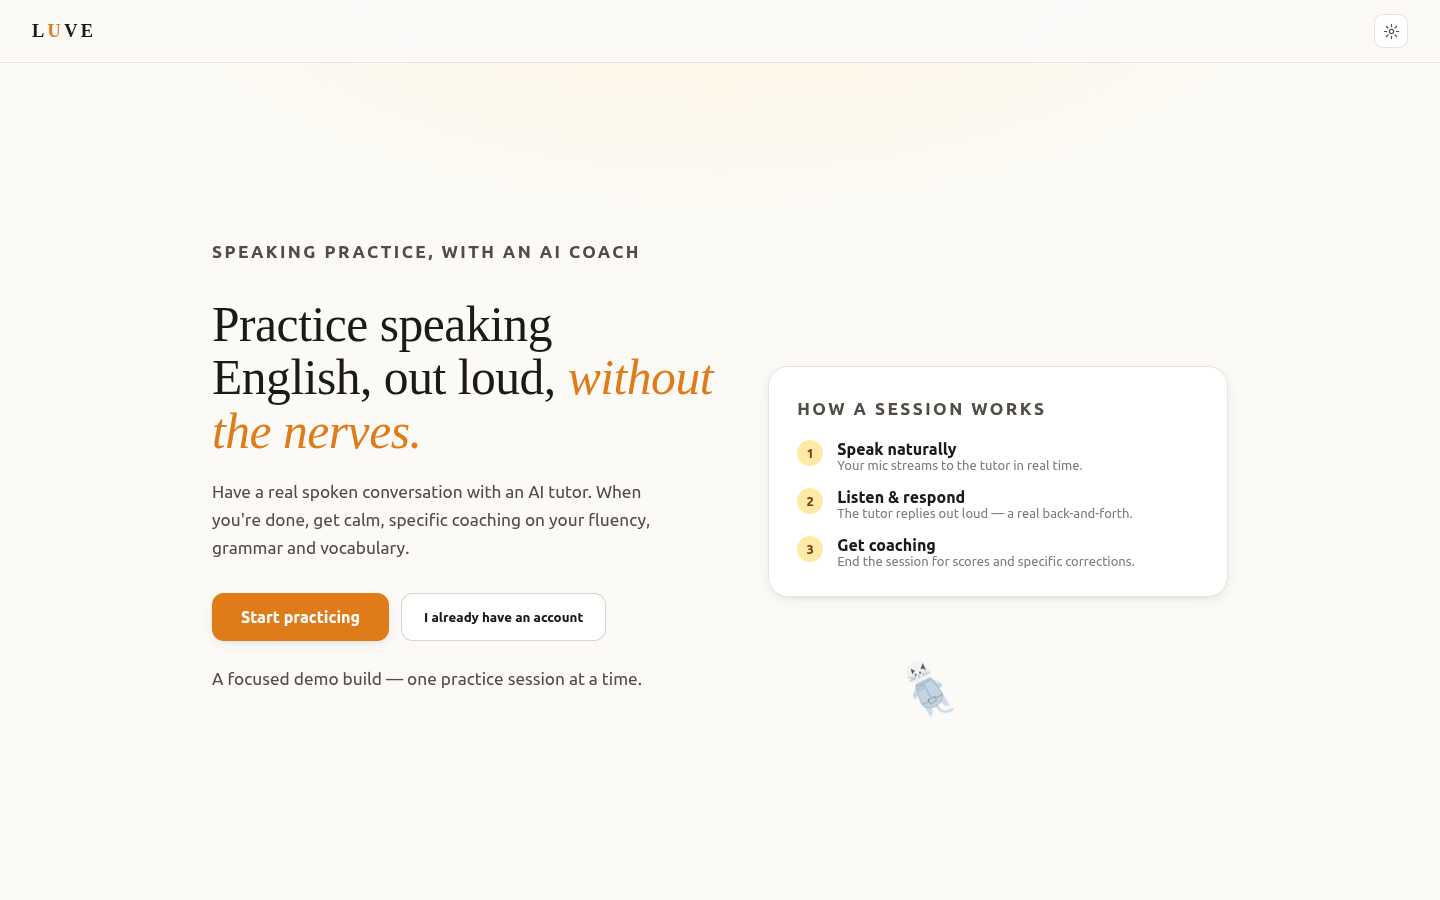
\includegraphics[width=\textwidth]{fig/ui_login.png}
  \caption{Authentication entry point of the baseline LUVE client.}
  \label{fig:ui-login}
\end{figure}

\textbf{Practice and real-time interface.} The practice screen is where the
learner initiates and controls a speaking session. From the design viewpoint,
this screen is responsible for starting a session, negotiating and maintaining
the WebRTC connection with the real-time gateway, and exchanging the audio and
control messages that drive the live conversation. During the session it
reflects the relevant interaction state to the learner --- for example, the
recognized speech and the tutor's conversational responses --- so that the
exchange is legible as it happens. Consistent with the system design, the
real-time interface presents conversational tutor replies only; grading is not
shown here because it is produced asynchronously after the session ends.

% TODO-FIGURE [VI]: Cần chụp màn hình giao diện luyện nói thời gian thực từ baseline main.
\begin{figure}[H]
  \centering
  % 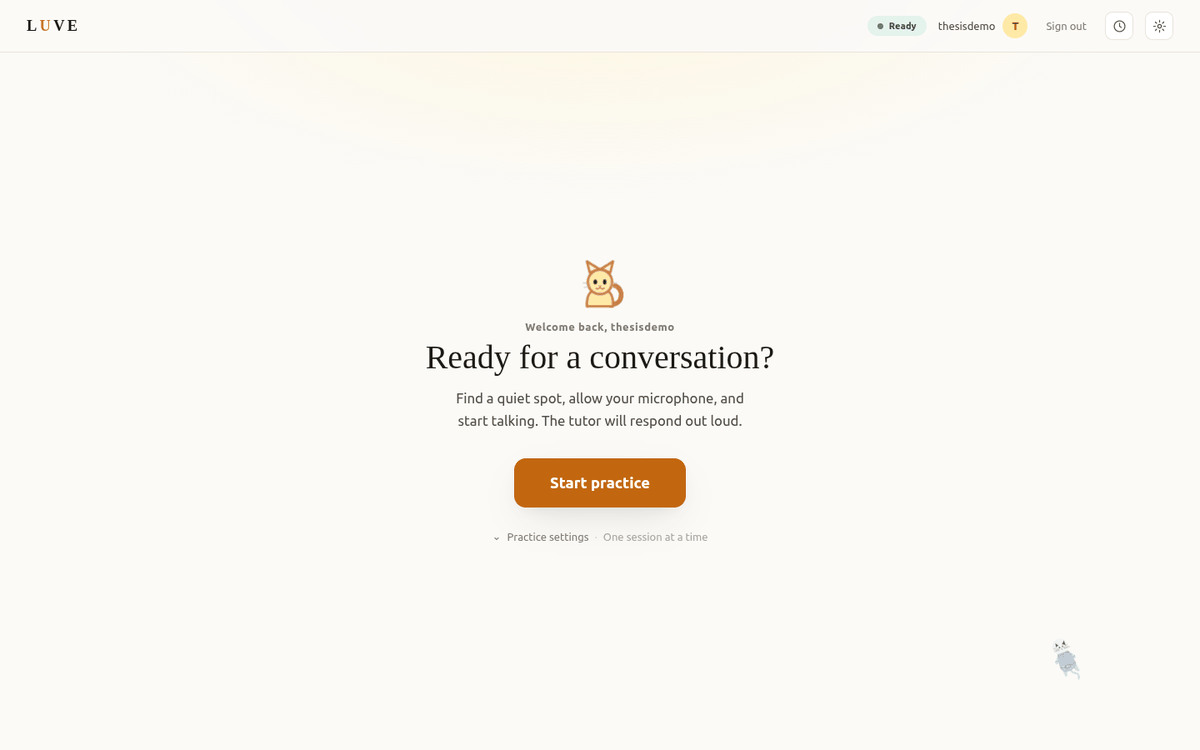
\includegraphics[width=\textwidth]{fig/ui_practice.png}
  \caption{Real-time practice screen of the baseline LUVE client.}
  \label{fig:ui-practice}
\end{figure}

\textbf{Saved-session and analysis interface.} After a session ends, the client
retrieves the learner's saved sessions and their grading results from the Core
API and presents them for review. Because grading runs asynchronously, a saved
session is not always accompanied by a result immediately, so the interface
distinguishes asynchronous states such as pending or processing grading,
available graded results, insufficient-evidence or skipped grading, and failed
or unavailable analysis. When a result is available, the interface displays the
overall and per-skill outcomes returned by the backend. When a
pronunciation-related value is returned, this thesis interprets it as a clarity
estimate derived from speech-recognition confidence and uncertainty, not as
acoustic or phoneme-level pronunciation scoring; the interface should avoid
presenting it as a true phoneme score. The default grading mode in the baseline
is an offline development-preview grader, so displayed scores must be understood
as demonstrative output rather than a real production assessment.

% TODO-FIGURE [VI]: Cần chụp màn hình giao diện saved session / grading result từ baseline main.
\begin{figure}[H]
  \centering
  % 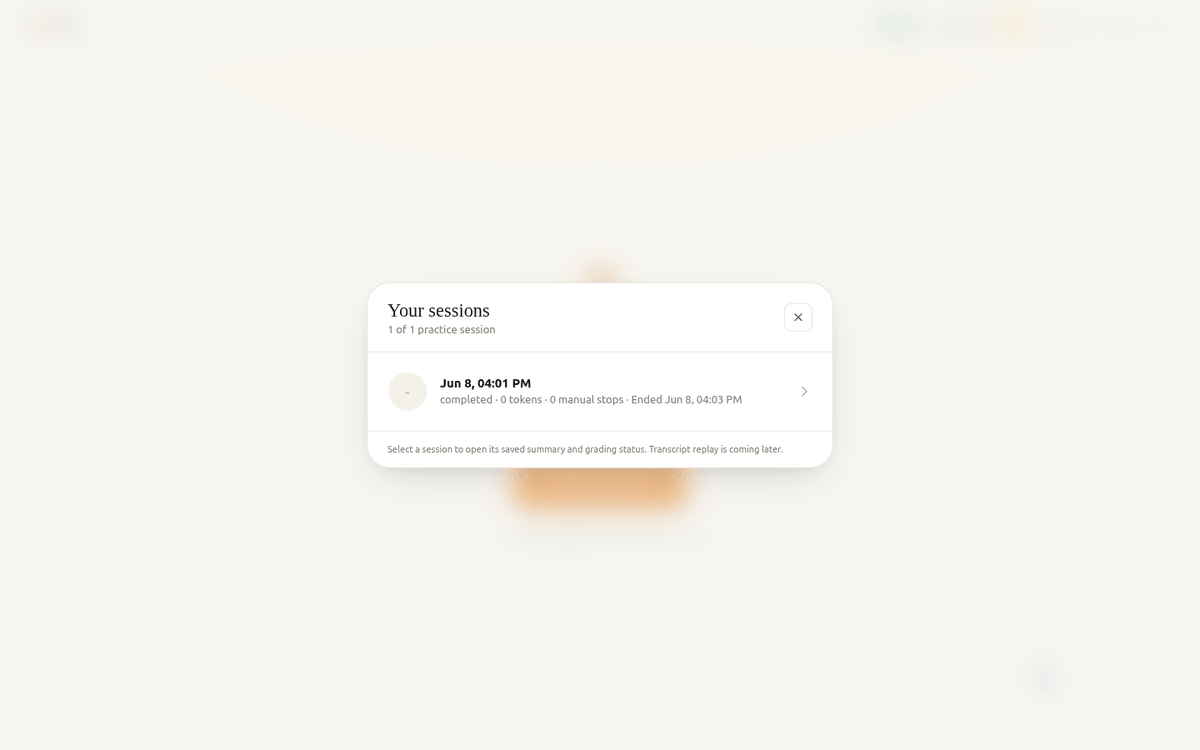
\includegraphics[width=\textwidth]{fig/ui_saved_session.png}
  \caption{Saved-session and grading-result screen of the baseline LUVE client.}
  \label{fig:ui-saved-session}
\end{figure}

\textbf{Error and state handling.} At the design level, the interface accounts
for the transitional and unavailable states that follow from the asynchronous
architecture. It handles a loading state while backend data is being fetched, a
pending state while grading for a completed session has not yet been produced,
and an unavailable state when analysis cannot be shown (for example, when
grading was skipped). These states keep the asynchronous boundary visible to
the learner instead of presenting an empty or misleading view.

\textbf{Scope limitation.} The interface described here is the baseline client
only. The ``cat companion'' interface and the associated mobile-layout
refinements introduced in PR~\#2 are not merged into \texttt{main} and are
therefore outside the scope of the implemented system discussed in this thesis.

\subsection{Algorithm and Processing Flow Design}

Rather than a single monolithic algorithm, LUVE is organized as a set of
cooperating processing flows that together realize an end-to-end speaking
practice session. This section describes those flows in terms of data flow,
control flow, and the boundaries between components. Five flows are presented:
the real-time speaking flow, the session lifecycle flow, the outbox and queue
flow, the asynchronous grading flow, and the retrieval/display flow. The
design deliberately keeps the latency-sensitive real-time work separate from
the deferred grading work, and the transitions between the two are mediated by
durable database state.

\textbf{Real-time speaking flow.} The real-time flow runs on the conversation
path between the browser and the TEN/WebRTC gateway. The browser captures the
learner's audio and exchanges audio and control messages with the gateway over
the WebRTC connection. The gateway manages the state of the active real-time
session and, where applicable, applies voice-activity detection (VAD) and
audio chunking to identify speech segments. Each segment is passed to the
speech-to-text (STT) component, which in the stable demo configuration runs in
\texttt{forced\_en} mode with the \texttt{small.en} model and second-pass
verification disabled, producing recognized text together with confidence
metrics. The recognized text is forwarded to the real-time LLM tutor, which
generates conversational replies only; it is not the grading component, and no
full scoring or pedagogical evaluation is produced on this path. Tutor
responses are returned to the learner through the TTS/WebRTC output path when
tutor audio is enabled. For
privacy, raw STT transcripts are not written to the application logs: following
the backend privacy patch (PR~\#1), log records retain only metadata such as
text length and confidence values.

% TODO-FIGURE [VI]: Cần vẽ sequence diagram cho luồng realtime: browser audio -> TEN/WebRTC gateway -> VAD/STT -> LLM tutor -> response/output.
\begin{figure}[H]
  \centering
  % 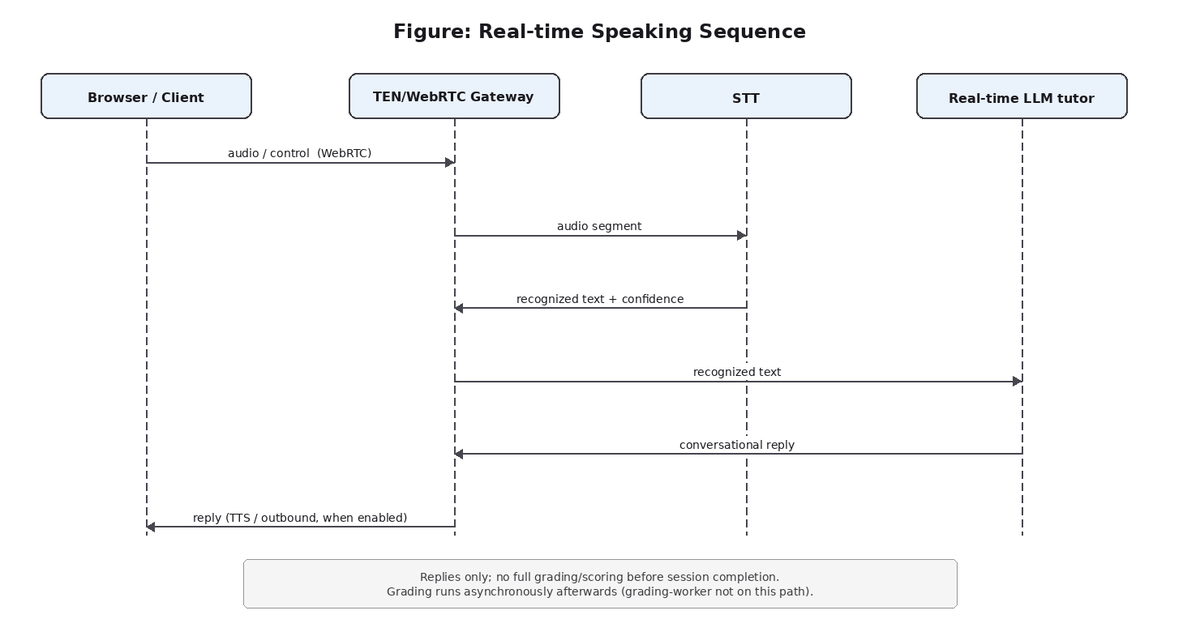
\includegraphics[width=\textwidth]{fig/realtime_sequence.png}
  \caption{Sequence of the real-time speaking flow (browser audio $\to$ gateway $\to$ VAD/STT $\to$ LLM tutor $\to$ output).}
  \label{fig:realtime-sequence}
\end{figure}

\textbf{Session lifecycle flow.} A practice session is created through the
Core API and, in the application flow, is associated with an authenticated
user. While the session is active, the real-time events it produces are
collected during the interaction. Durable persistence happens at completion:
when the session ends, the system records the session state and the
information needed for downstream processing. Because events are accumulated in
memory during the interaction and persisted only at completion, a process
crash before completion may lose the portion of the event log not yet written;
this is an accepted limitation of the current prototype. Completion is also the
point at which downstream grading work is created and scheduled, which links
this flow to the outbox and queue flow below.

\textbf{Outbox and queue flow.} The hand-off from a completed session to the
grading pipeline is built on a durable outbox. The \texttt{session\_outbox}
table is an ordinary PostgreSQL table, not a standalone queue service. At
completion, the session state update and the corresponding outbox row are
committed together in a single database transaction, so the intent to grade is
recorded durably and atomically with the session itself. After the commit, the
system attempts an inline publish of the \texttt{session.completed} event to
RabbitMQ. If the publish fails, a warning is logged and the durable outbox row
remains in place for later recovery. The outbox relay that would automatically
re-deliver pending rows is disabled by default, so recovery after a failed
publish is a manual operation unless the relay is enabled. The mechanism is
oriented toward at-least-once delivery rather than exactly-once; to keep this
safe, downstream processing is idempotent and deduplicated at the session
level, so a re-delivered event does not produce duplicate results.

% TODO-FIGURE [VI]: Cần vẽ flowchart xử lý lỗi publish RabbitMQ: commit DB thành công -> publish fail -> warning log -> outbox row chờ relay/manual recovery.
\begin{figure}[H]
  \centering
  % 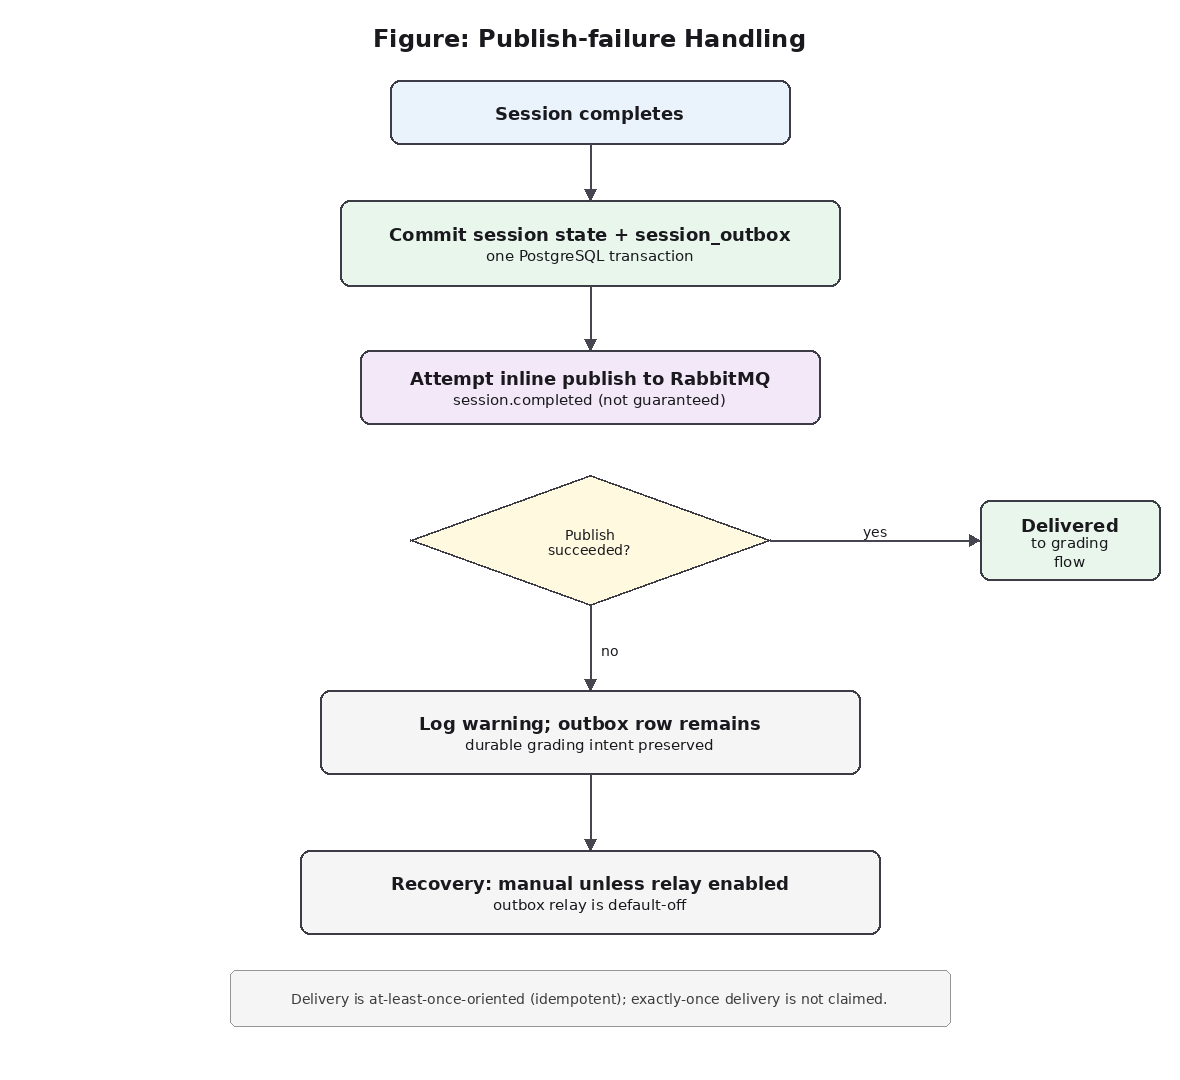
\includegraphics[width=\textwidth]{fig/publish_failure_flow.png}
  \caption{Publish-failure handling (DB commit succeeds $\to$ publish fails $\to$ warning logged $\to$ outbox row awaits relay/manual recovery).}
  \label{fig:publish-failure-flow}
\end{figure}

\textbf{Asynchronous grading flow.} Grading runs off the real-time path. The
grading-worker consumes the \texttt{session.completed} work item delivered
through the queue, reads the completed session and its transcript evidence, and
produces a grading outcome. When grading succeeds, it writes a
\texttt{grading\_results} row; when grading cannot proceed or is intentionally
skipped (for example, when eligibility conditions are not met), it records a
\texttt{grading\_skip\_log} entry instead. The system supports two grading
modes: an offline \emph{fake} (development-preview) grader, which is the
default, and a real LLM-based grader that can be enabled by configuration.
Among the reported skills, the pronunciation score is a clarity estimate
derived from STT confidence and uncertainty signals, not an acoustic or
phoneme-level pronunciation analysis.

% TODO-FIGURE [VI]: Cần vẽ sequence diagram cho luồng hoàn tất phiên và chấm điểm: session completed -> session_outbox -> RabbitMQ -> grading-worker -> grading_results.
\begin{figure}[H]
  \centering
  % 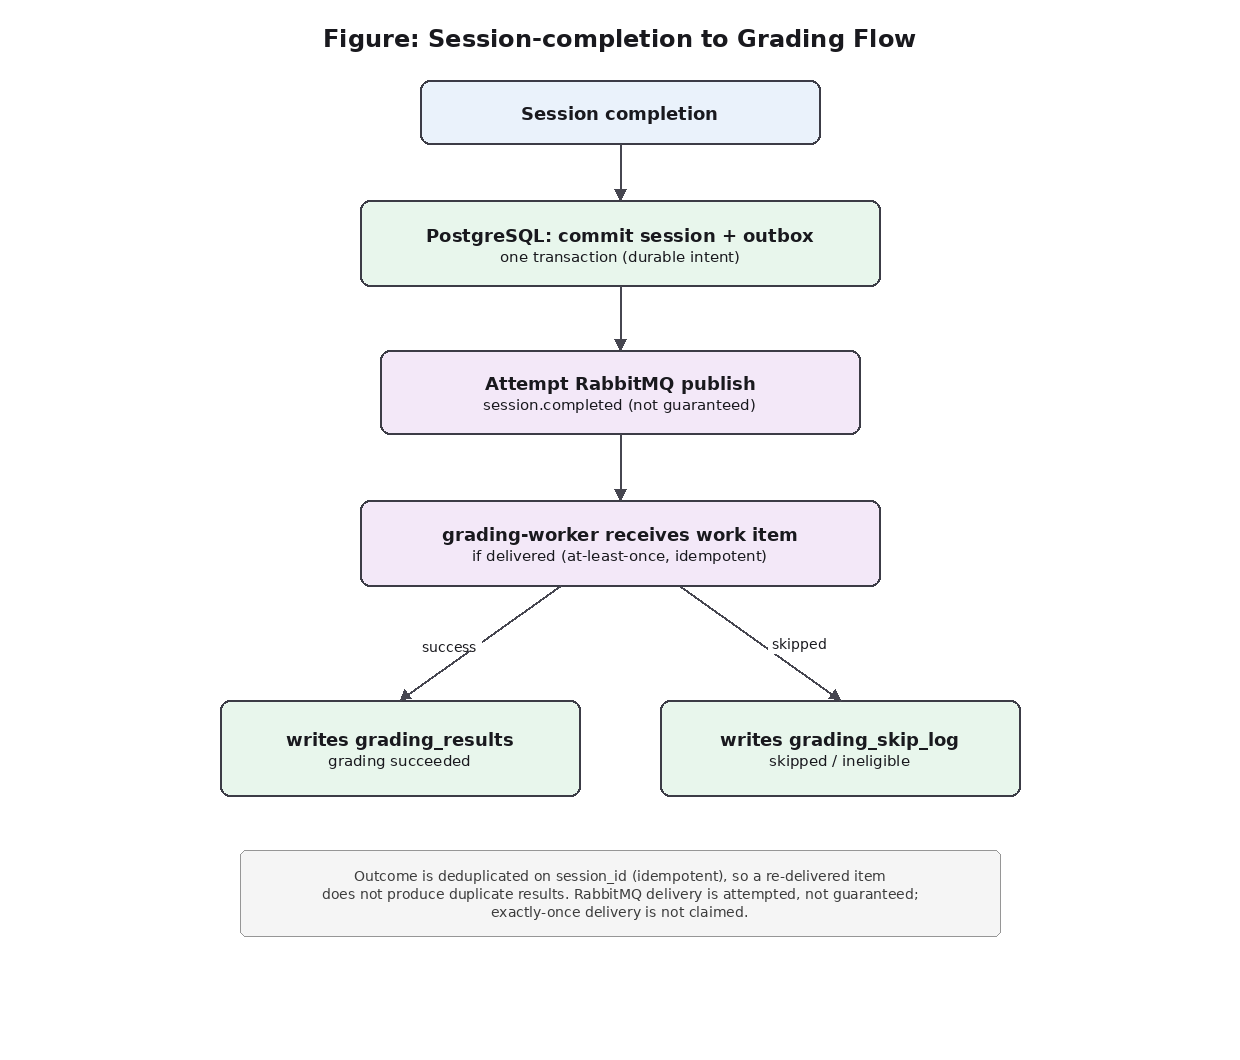
\includegraphics[width=\textwidth]{fig/session_grading_flow.png}
  \caption{Flow from session completion to grading (session\_outbox $\to$ RabbitMQ $\to$ grading-worker $\to$ grading\_results).}
  \label{fig:session-grading-flow}
\end{figure}

\textbf{Retrieval and display flow.} Grading is not synchronous with the
conversation, so results become available after the session ends. The client
later retrieves saved sessions and their grading results from the Core API for
display to the learner. The detailed user-interface design is covered
separately in the Interface Design section; here it is sufficient to note that
the retrieval path reads persisted records rather than participating in the
real-time pipeline.

\textbf{Failure and limitation notes.} The processing flows above operate
within the controlled-demo, research-prototype scope of the system. Several
constraints follow from this scope and shape the design. Schema changes rely on
numbered manual SQL migration files with manual verification; there is no
production-grade automatic migration runner. Readiness and observability are
limited --- health checks are shallow and there is no dedicated metrics
endpoint --- so operational state is inferred largely from logs. The real-time
path is capped at a single session per node, and horizontal scaling is not
claimed or demonstrated. The STT configuration is English-focused
(\texttt{forced\_en} with \texttt{small.en}); stable multilingual recognition
is not claimed. Likewise, the system does not claim exactly-once delivery or
acoustic/phoneme-level pronunciation scoring. These limitations are revisited
in Chapter~5.

\section{Chapter Summary}
% [PLACEHOLDER]

% ------------------- CHAPTER 4 ------------------------------------
\chapter{IMPLEMENTATION AND RESULTS}

\section{Development Environment}
% [PLACEHOLDER] Docker Compose monorepo; Python/FastAPI; PostgreSQL; RabbitMQ;
% Vite/React/TypeScript client. Frozen baseline: main@6a61bc8.
% TODO-TABLE [VI]: Bảng 4.1 - Công nghệ và môi trường phát triển. Nội dung cần có:
% thành phần (ngôn ngữ, framework, CSDL, message broker, STT, client, container),
% tên/phiên bản, vai trò.
% TODO-TABLE [VI]: Bảng 4.2 - Cấu hình demo STT/grading. Nội dung cần có:
% STT model=small.en, mode=forced_en, second-pass=tắt; GRADING_PROVIDER=fake (mặc định),
% GRADING_FAKE_FALLBACK=tắt, OUTBOX_RELAY_ENABLED=false. Bám đúng LUVE_FACTS.md.

\section{Implementation Process}
\subsection{Core Module Implementation}
% [PLACEHOLDER] core-api (REST + gateway), grading-worker.
\subsection{Data Processing}
% [PLACEHOLDER] STT -> analysis -> session saving -> grading.

\section{Achieved Results}
\subsection{Program Execution Results}
% [PLACEHOLDER] End-to-end demo; screenshots.
% TODO-FIGURE [VI]: fig/demo_session — ảnh chụp một phiên luyện nói (chạy thật).
\begin{figure}[H]
  \centering
  % 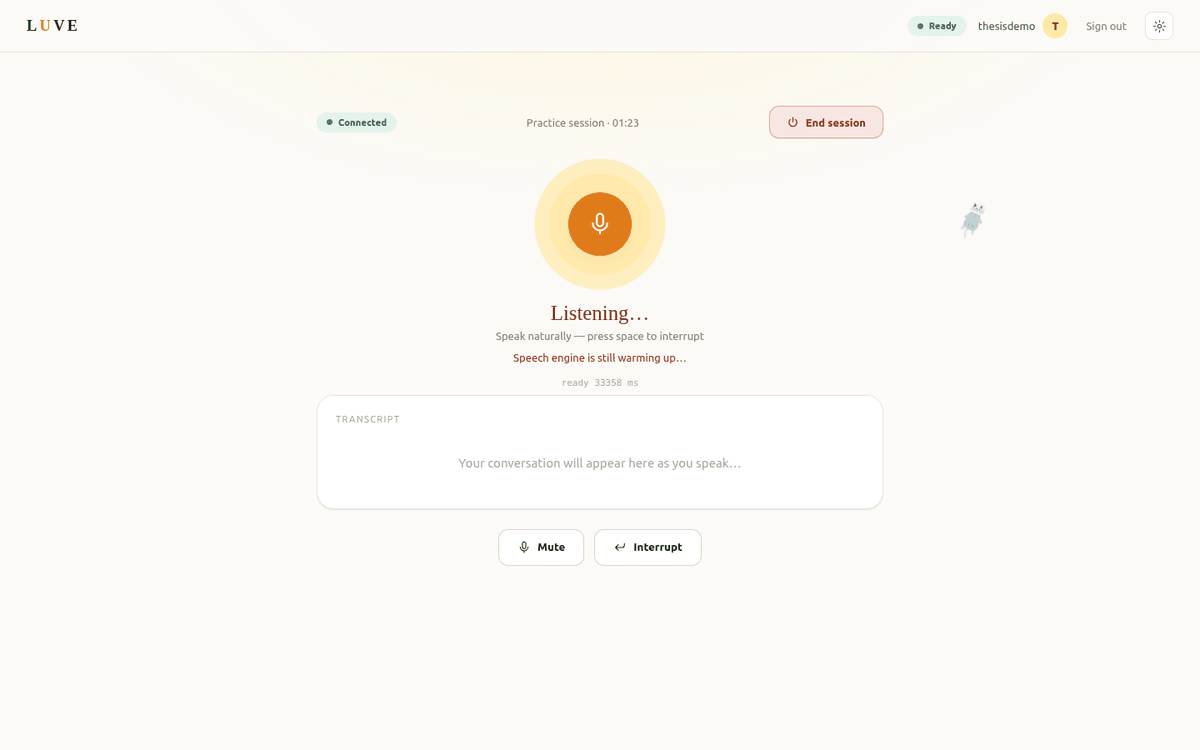
\includegraphics[width=\textwidth]{fig/demo_session.png}
  \caption{Demo result: a real-time practice session.}
  \label{fig:demo-session}
\end{figure}
% TODO-FIGURE [VI]: fig/demo_grading — bảng điểm phiên đã lưu (chạy thật).
\begin{figure}[H]
  \centering
  % 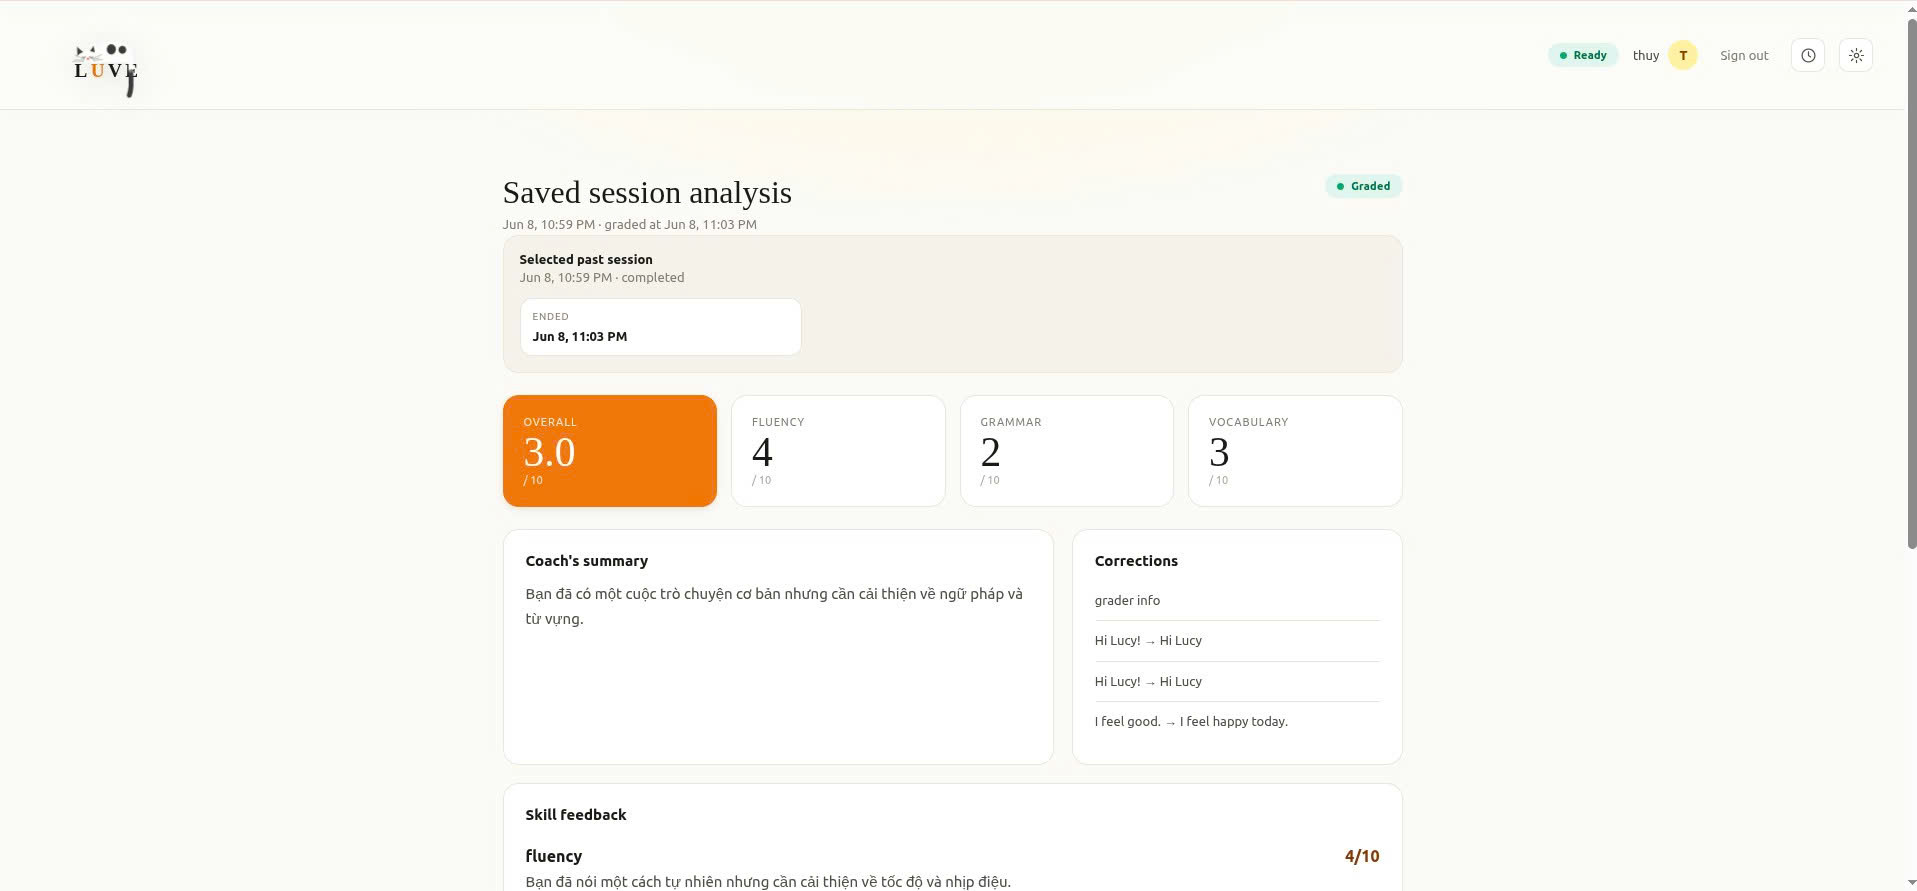
\includegraphics[width=\textwidth]{fig/demo_grading.png}
  \caption{Demo result: grading panel for a saved session.}
  \label{fig:demo-grading}
\end{figure}
\subsection{Result Evaluation}
% [PLACEHOLDER] Do NOT fabricate evaluation figures. Report only actually
% measured results.

\section{Testing}
% [PLACEHOLDER] Describe real testing (per-service pytest, smoke tests).
% Honest note: the full test suite has intermittently hung in some
% environments; there is no CI gate yet.
% TODO-TABLE [VI]: Bảng 4.3 - Kiểm thử/smoke test. Nội dung cần có: hạng mục kiểm thử,
% lệnh/cách chạy, kết quả thực tế. CHỈ điền kết quả thật, không bịa.

\section{Chapter Summary}
% [PLACEHOLDER]

% ------------------- CHAPTER 5 ------------------------------------
\chapter{CONCLUSION AND FUTURE WORK}

\section{Conclusion}
% [PLACEHOLDER]

\section{Thesis Contributions}
% [PLACEHOLDER]

\section{Limitations}
% [PLACEHOLDER] Follow the "Known limitations" section of LUVE_FACTS.md:
% controlled-demo; English-forced STT; pronunciation is a clarity estimate
% from STT confidence, not phoneme scoring; durable outbox but relay default-off;
% no production migration runner; shallow health/observability; single-session-per-node.
% TODO-TABLE [VI]: Bảng 5.1 - Hạn chế và hướng phát triển. Nội dung cần có:
% hạn chế hiện tại (từ LUVE_FACTS.md), hướng khắc phục/phát triển tương ứng.

\section{Future Work}
% [PLACEHOLDER]

% ===================== REFERENCES =================================
\printbibliography[heading=bibintoc,title={REFERENCES}]
% Note: IEEE style is configured (style=ieee). Add \cite{...} in the text
% and declare the matching entry in refs.bib. Do NOT fabricate references.

% ===================== APPENDICES ================================
% \appendix switches \chaptername to \appendixname ("APPENDIX") and numbers
% chapters A, B, C. Using real chapters (not starred sections) so each
% appendix appears in the table of contents automatically.
\appendix

\chapter{Source Code}
% [PLACEHOLDER] Insert important source-code excerpts (if needed).
% Example listing skeleton:
% \begin{lstlisting}[language=Python]
% # ...
% \end{lstlisting}

\chapter{Survey Results}
% [PLACEHOLDER]
% TODO-TABLE [VI]: Bảng B.1 - Kết quả khảo sát. Nội dung cần có: câu hỏi khảo sát,
% số người tham gia, kết quả tổng hợp. KHÔNG bịa số liệu — chỉ điền khi có dữ liệu thật.

\chapter{User Guide}
% [PLACEHOLDER] Installation and run guide (docker compose --profile app up -d --build).

\end{document}
